\begin{figure}[t!]
  \centering
  \begin{subfigure}[t]{0.3\textwidth}
    \centering
    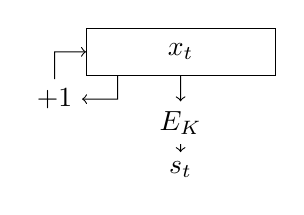
\begin{tikzpicture}[xscale=0.8,yscale=0.6]
      \draw (0, 0) rectangle (3, 1) node[pos=0.5]{$x_t$};
      \draw (1.5, -1) node(bc){$E_K$} ;
      \draw (1.5, -2) node(s){$s_t$} ;
      \draw (-0.5, -0.5) node(add){$+1$} ;
      \draw[->] (1.5, 0) -- (bc) ;
      \draw[->] (bc) -- (s) ;
      \draw[->] (0.5, 0) -- (0.5, -0.5) -- (add) ;
      \draw[->] (add) -- (-0.5, 0.5) -- (0, 0.5) ;
    \end{tikzpicture}
    \caption{\label{fig:counter-mode}Counter mode.}
  \end{subfigure}
  \hfill
  \begin{subfigure}[t]{0.3\textwidth}
    \centering
    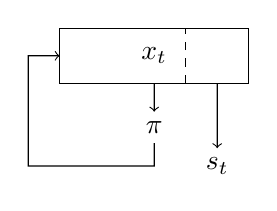
\begin{tikzpicture}[xscale=0.8,yscale=0.7]
      \draw (0, 0) rectangle (3, 1) node[pos=0.5]{$x_t$};
      \draw (1.5, -0.8) node(bc){$\pi$} ;
      \draw (2.5, -1.5) node(s){$s_t$} ;
      \draw[->] (1.5, 0) -- (bc) ;
      \draw[->] (bc) -- (1.5, -1.5) -- (-0.5, -1.5) -- (-0.5, 0.5) -- (0, 0.5) ;
      \draw[style=dashed] (2, 0) -- (2, 1) ;
      \draw[->] (2.5, 0) -- (s) ;
    \end{tikzpicture}    
    \caption{\label{fig:sponge-mode}Permutation-based.}
  \end{subfigure}
  \hfill
  \begin{subfigure}[t]{0.35\textwidth}
    \centering
    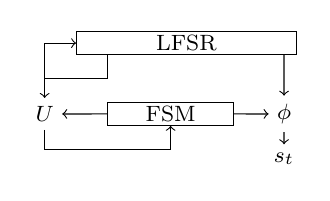
\begin{tikzpicture}[xscale=0.8,yscale=0.6]
      \footnotesize
      \draw (0.5, 0) rectangle (4, 0.5) node[pos=0.5]{LFSR} ;
      \draw (1, -1.5) rectangle (3, -1) node[pos=0.5]{FSM} ;
      \draw (0, -1.25) node(nl){$U$} ;
      \draw (3.8, -1.25) node(phi){$\phi$} ;
      \draw (3.8, -2.2) node(s){$s_t$} ;
      \draw[->] (1, 0) -- (1, -0.5) -- (0, -0.5) -- (0, 0.25) -- (0.5, 0.25) ;
      \draw[->] (0, -0.5) -- (nl) ;
      \draw[->] (1, -1.25) -- (nl) ;
      \draw[->] (nl) -- (0, -2) -- (2, -2) -- (2, -1.5) ;
      \draw[->] (3, -1.25) -- (phi) ;
      \draw[->] (3.8, 0) -- (phi) ;
      \draw[->] (phi) -- (s) ;
    \end{tikzpicture}    
    \caption{\label{fig:classical-stream}LFSR and FSM.}
  \end{subfigure}
  \caption{Different types of stream cipher structures.}
  \label{fig:streams}
\end{figure}


% Leo: ce qui suit est pour qu'emacs compile bien l'article, pas touche !
%%% Local Variables:
%%% mode: latex
%%% ispell-local-dictionary: "english"
%%% TeX-master: "../main"
%%% End:



